\section{Aplicação}


\subsection{Funcionamento}

Ao abrir a aplicação na página web podemos ver a página mostrada abaixo. Esta mostra alguns filmes presentes no nosso sistema de recomendação, que alternam entre si a cada 4 segundos desde que o utilizador não tenha o rato em cima de um. Esta página permite fazer o registo de um novo utilizador ou que este faça o login, caso já tenha conta.\newline

\begin{figure}[H]
\centering
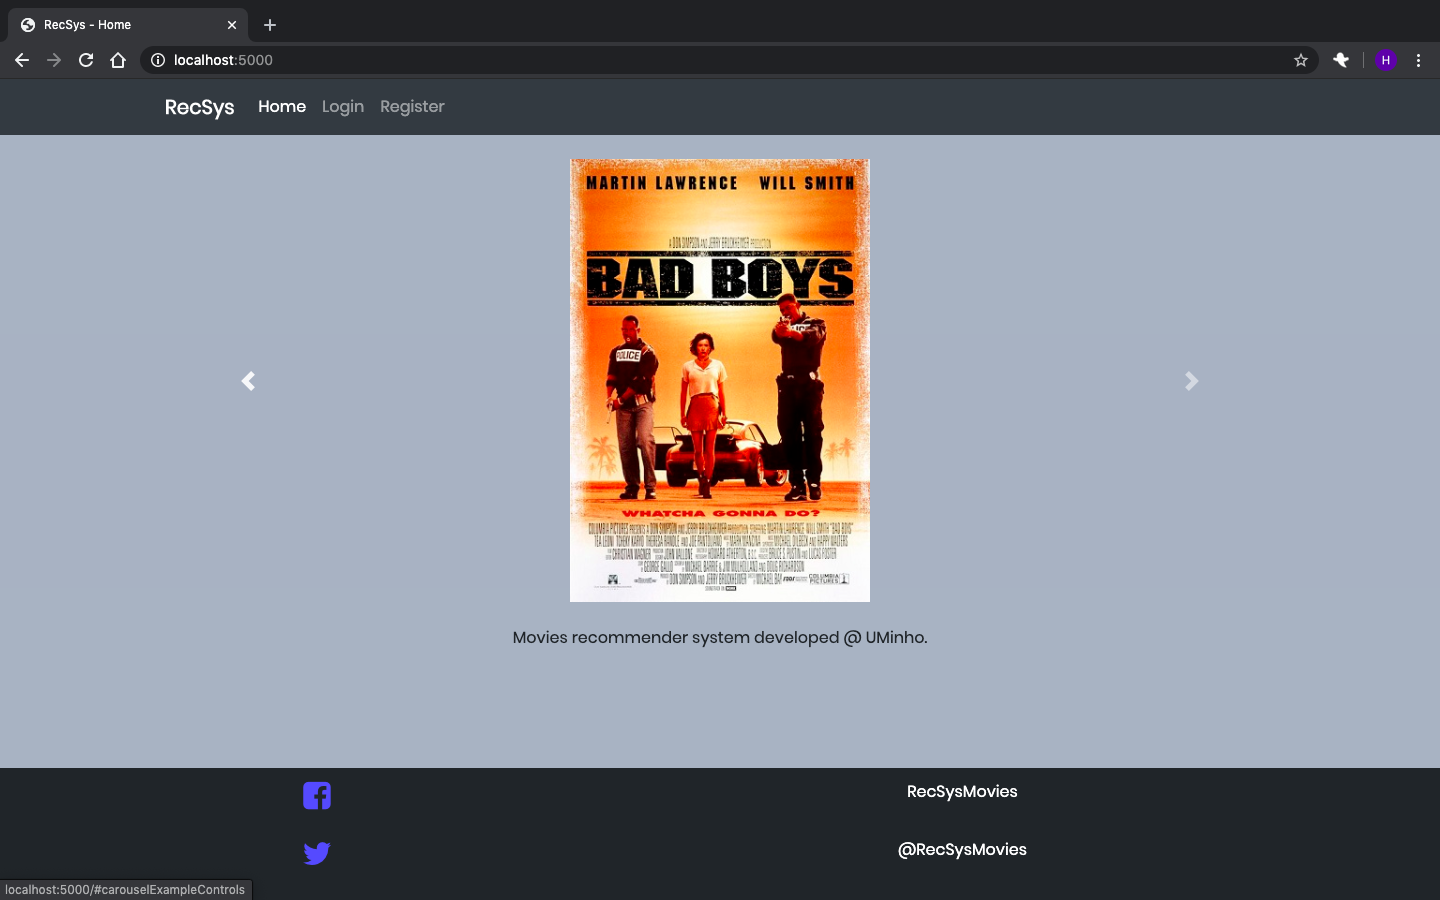
\includegraphics[width=\textwidth]{1.png}
\caption {Homepage RecSys}
\label {fig07}
\end{figure}

Caso não tenhamos conta temos de fazer o registo. Neste temos de inserir um nome de utilizador, um email válido e uma password.  Ao inserir na base de dados um id é gerado para o utilizador e inserido no campo id do documento na coleção users.\newline

\begin{figure}[H]
\centering
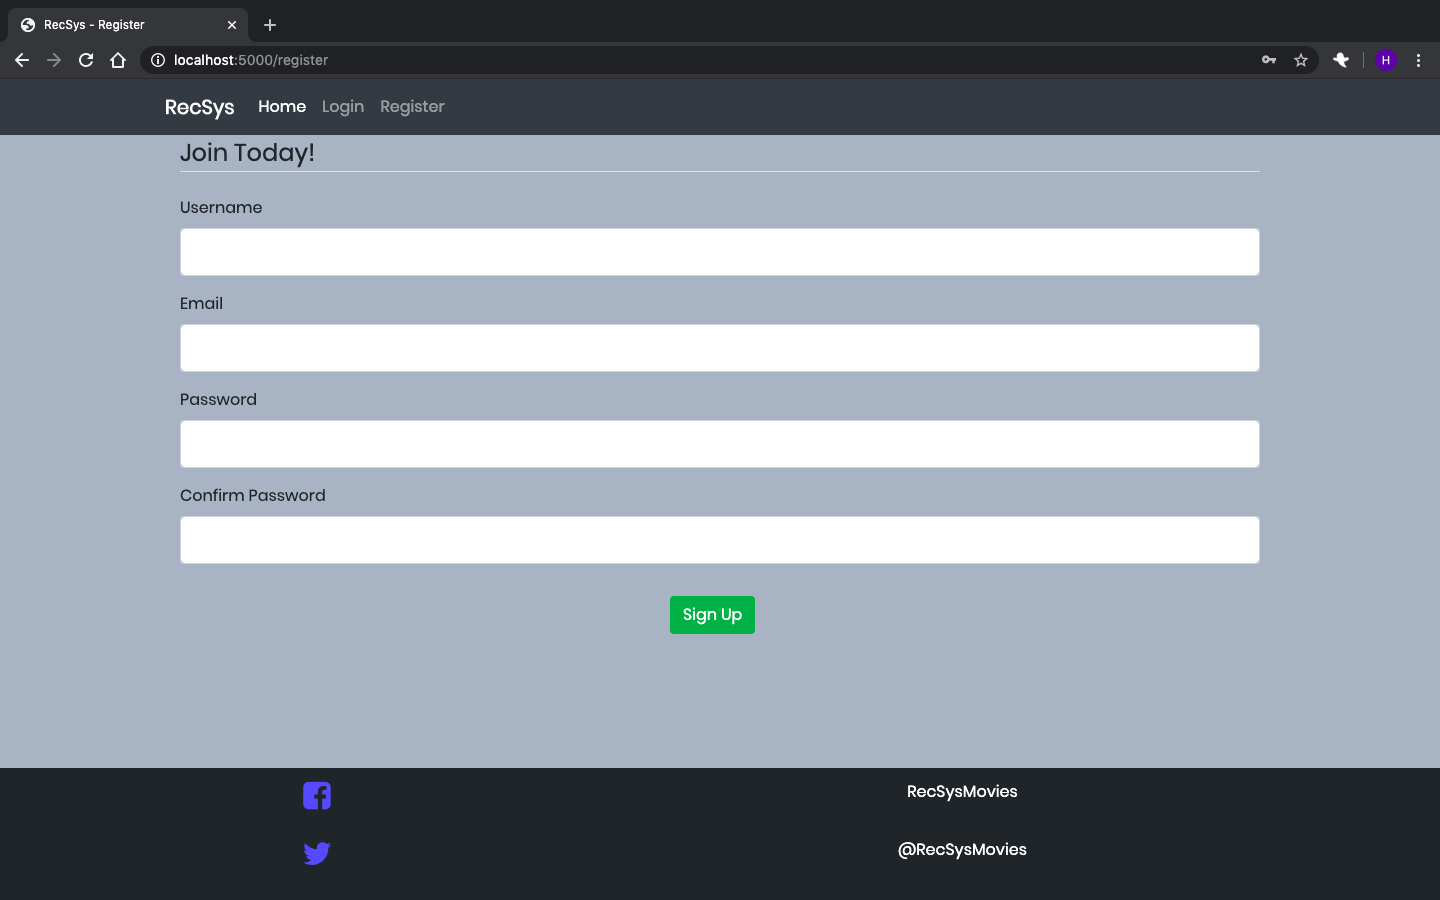
\includegraphics[width=\textwidth]{registo.png}
\caption {Register Page RecSys}
\label {fig08}
\end{figure}

\begin{figure}[H]
Caso já tenhamos conta devemos efetuar o login inserindo o email e a password.\newline

\centering
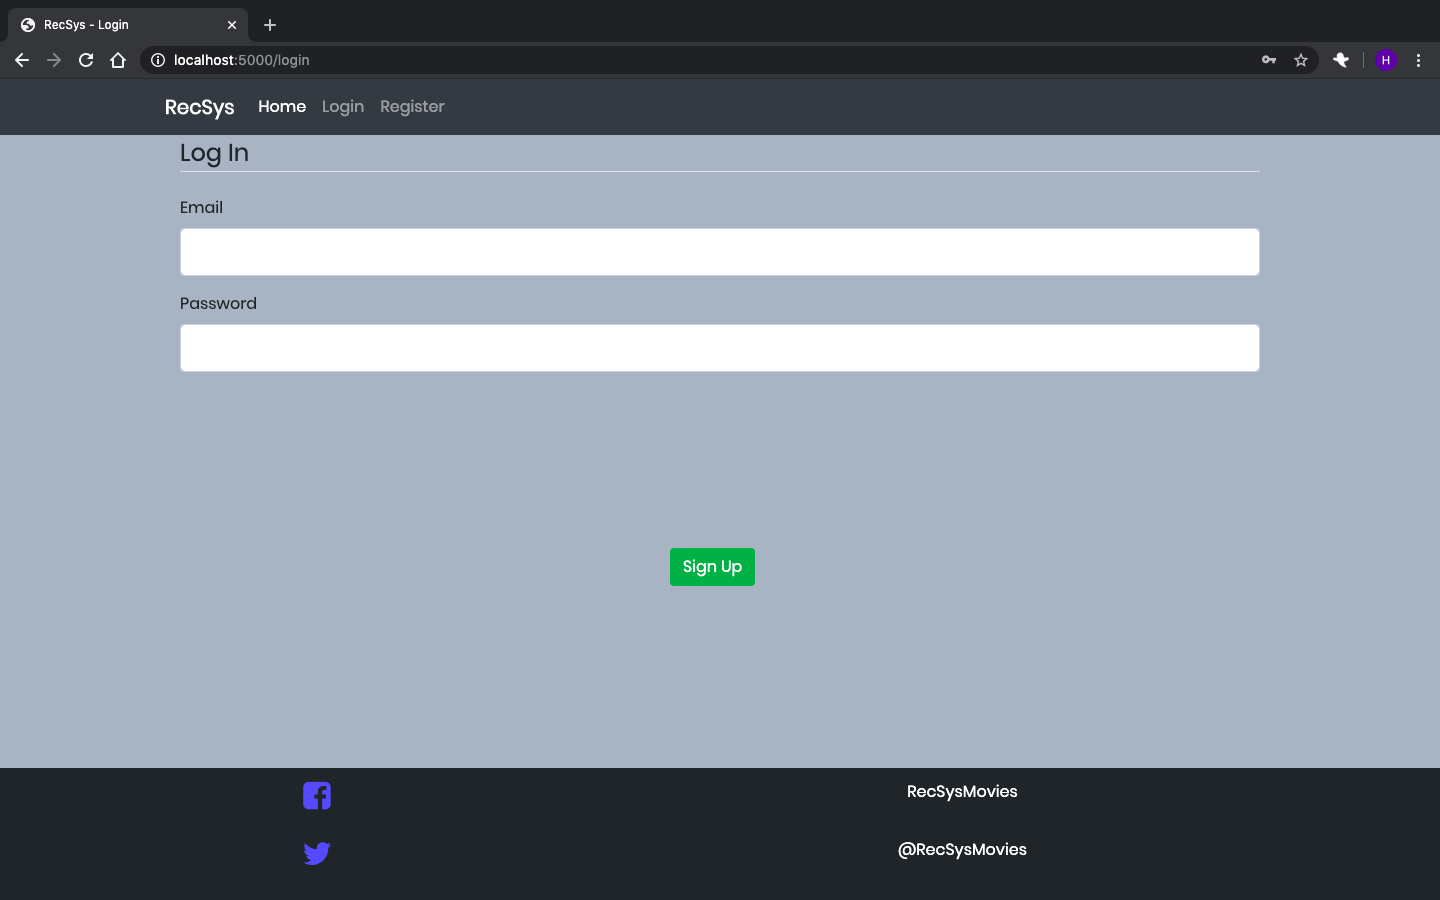
\includegraphics[width=\textwidth]{2.png}
\caption {Login Page RecSys}
\label {fig09}
\end{figure}

Quando um utilizador efetua o login com sucesso na sua conta pode ver os filmes que foram recentemente adicionados à nossa coleção(são os filmes com menos votações da nossa base de dados e são ordenados por data caso o número de votações coincida). Este sistema funciona graças ao sistema implementado na função filmsColdCases() que promove os filmes que não têm como ser recomendados de outra forma por falta de avaliações de utilizadores.\newline


\begin{figure}[H]
\centering
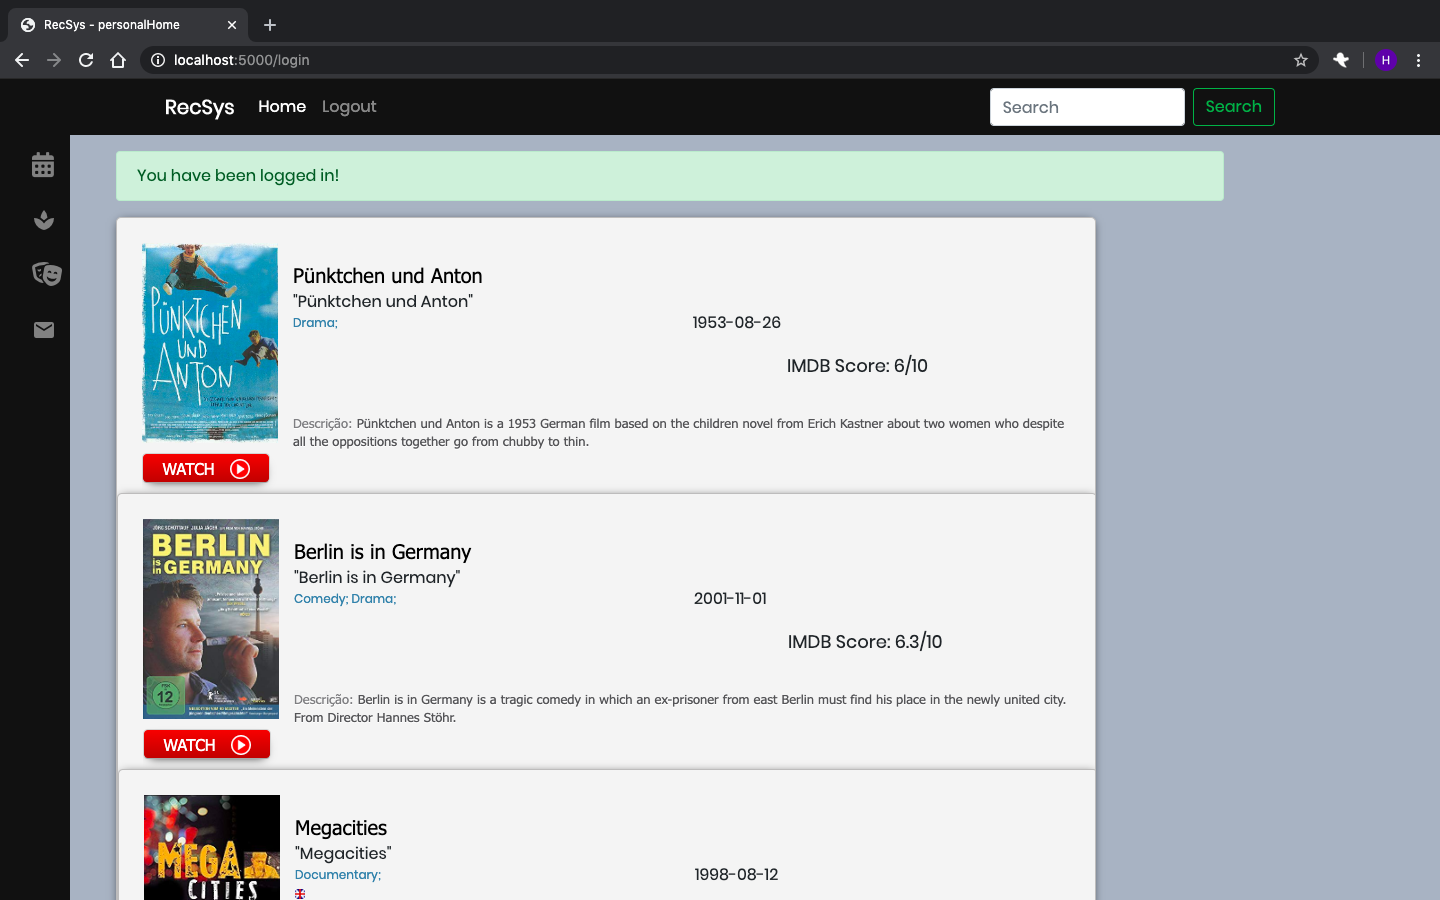
\includegraphics[width=\textwidth]{ColdFilms.png}
\caption {Start Page RecSys}
\label {fig10}
\end{figure}

Adicionalmente é possivel através desta página pesquizar filmes por ano de lançamento (apenas são mostrados anos de filmes presentes na base de dados), por género e por um dos sistemas de recomendação disponibilizados.\newline


\begin{figure}[H]
\centering
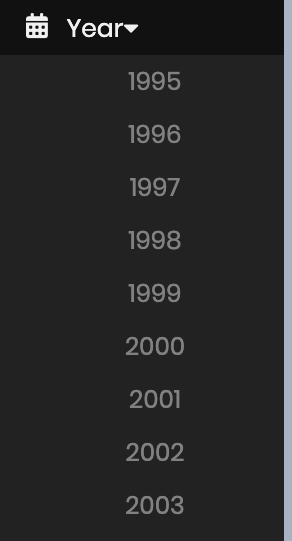
\includegraphics[scale=0.25]{7.png}
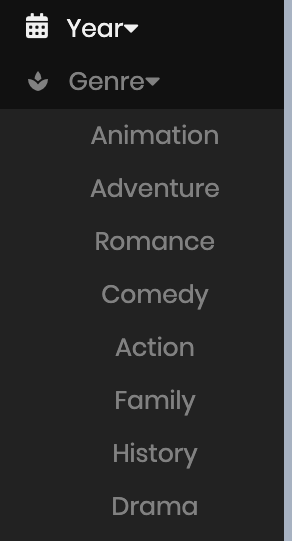
\includegraphics[scale=0.25]{8.png}
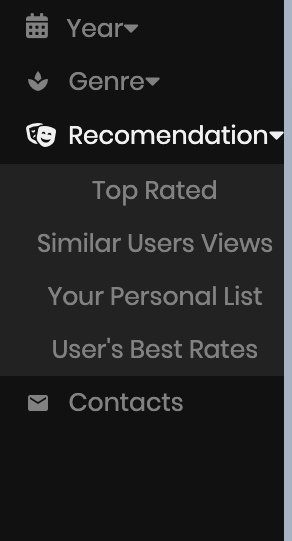
\includegraphics[scale=0.25]{9.png}
\caption {Year, Genre and Recomendation Search options RecSys}
\label {fig11}
\end{figure}

Uma alternativa para procurar filmes é utilizar a \textit{search bar} disponibilizada, onde o utilizador introduz uma palavra, frase, ou expressão e todos os filmes com essa palavra/frase/expressão associada são apresentados.\newline

\begin{figure}[H]
\centering
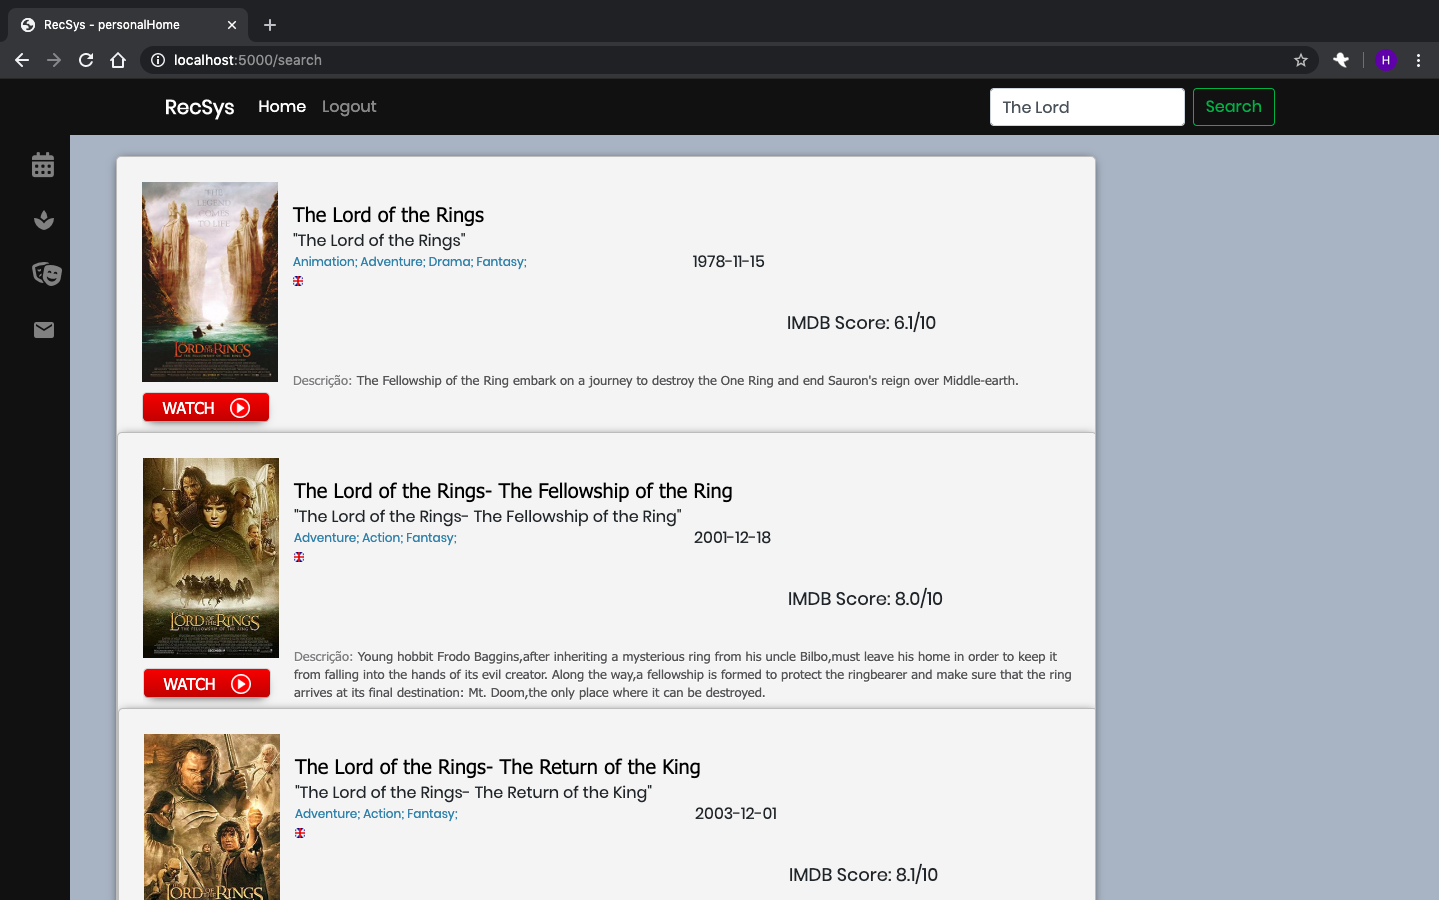
\includegraphics[width=\textwidth]{5.png}
\caption {Search Bar Results Page RecSys}
\label {fig12}
\end{figure}

Após visualizar o filme, o utilizador poderá atribuir uma pontuação (1 a 5 estrelas). Note-se que o botão submit fica bloqueado até uma classificação ser escolhida.

\begin{figure}[H]
\centering
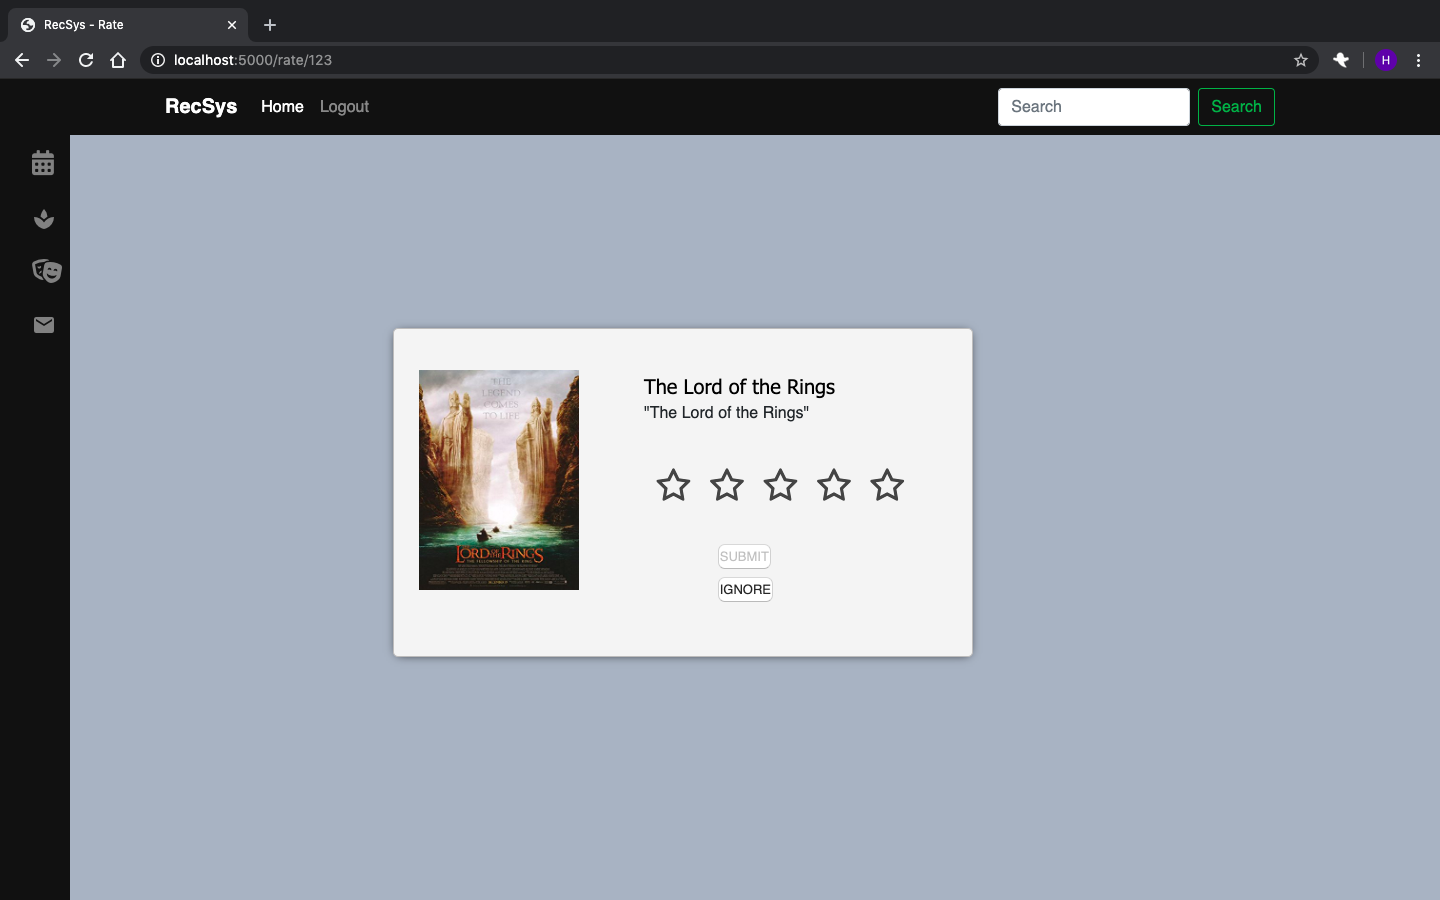
\includegraphics[width=\textwidth]{ignore.png}
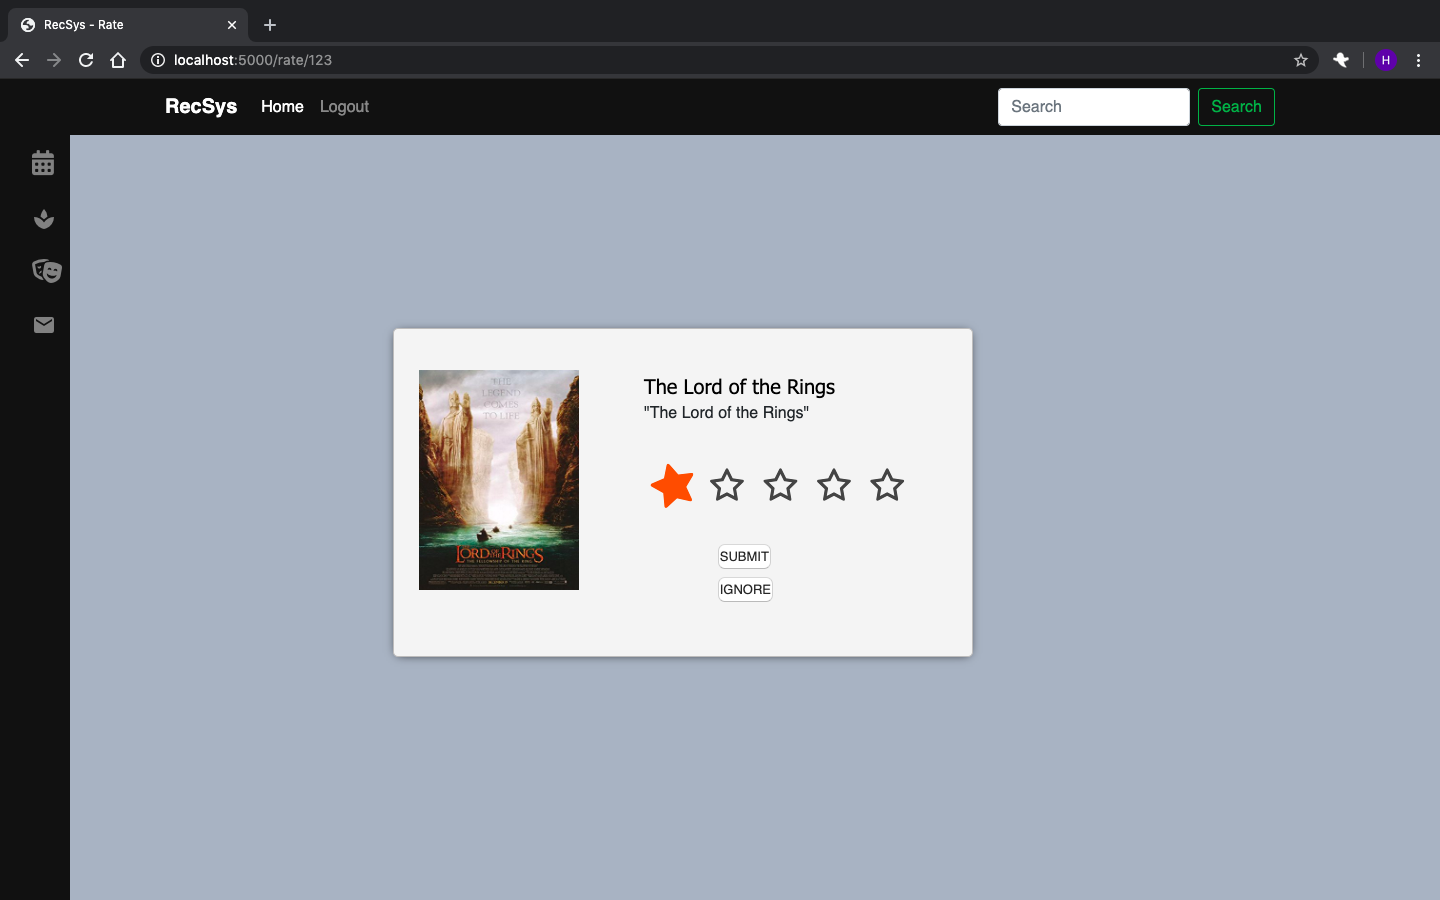
\includegraphics[width=\textwidth]{11.png}
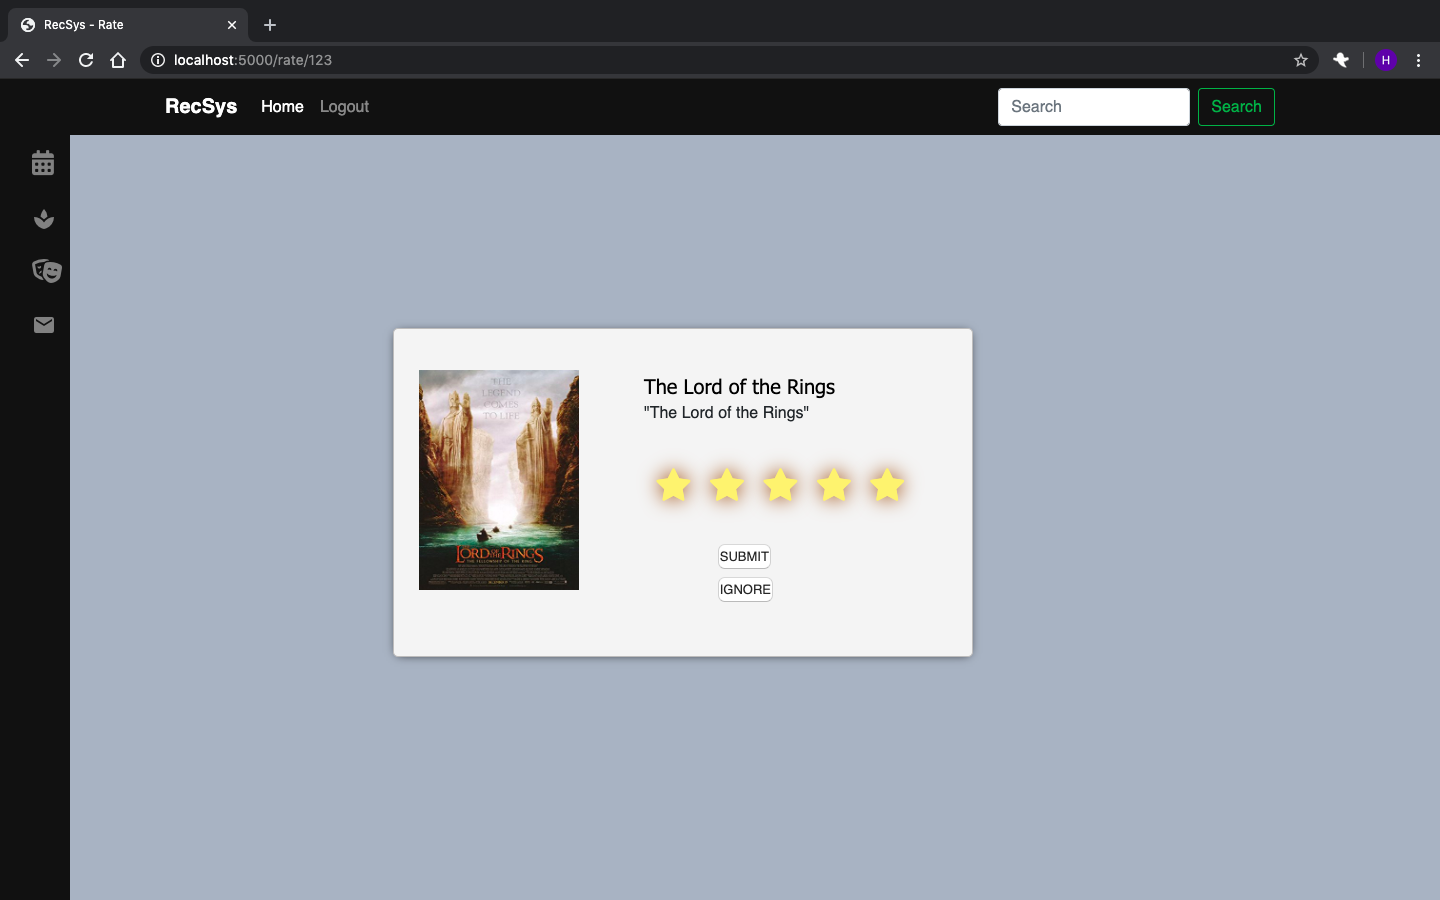
\includegraphics[width=\textwidth]{12.png}
\caption {Rating Page RecSys}
\label {fig13}
\end{figure}


Sempre que um utilizador atribui uma pontuação a um filme é adicionada essa informação à base de dados na coleção userRating. Por exemplo, se um utilizador x que viu um filme y e atribuiu uma pontuação z, esta a informação fica guardada na forma {"\_id" : ObjectId(....), "userId" : x, "movieId" : y, "rating" : z, "timestamp" : ...}.\newline


\par Se escolhermos o sistema de recomendação \textit{"Top Rated"}, obteremos os 10 melhores filmes segundo a IMDB ordenados por ordem decrescente de nota.\newline


\begin{figure}[H]
\centering
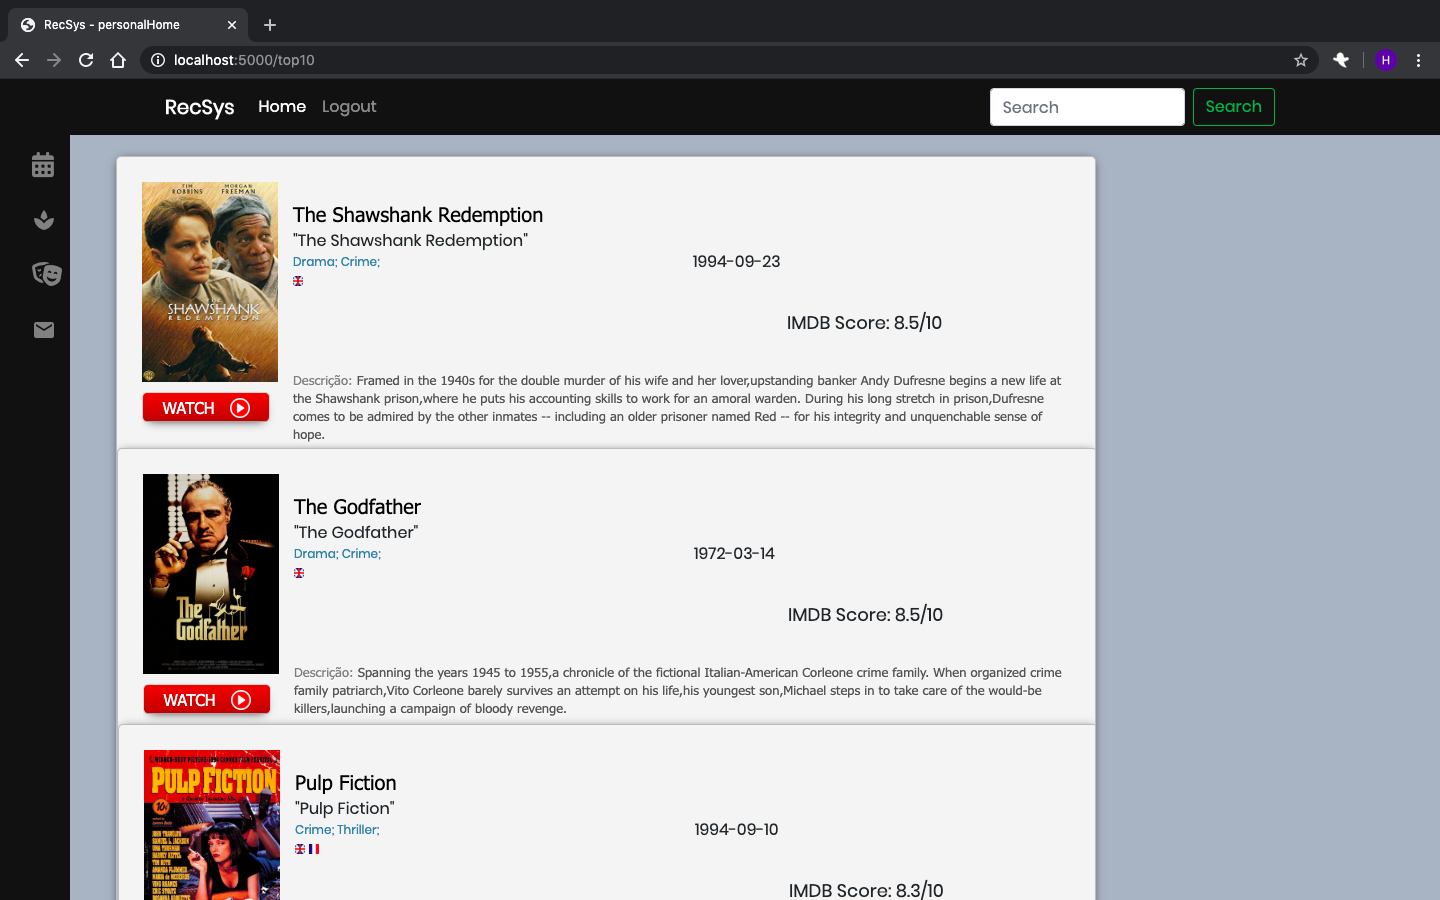
\includegraphics[width=\textwidth]{top10.png}
\caption {Top Rated Page RecSys}
\label {fig14}
\end{figure}

Se escolhermos o sistema de recomendação \textit{"Similar User's Views"}, obtemos os filmes mais bem cotados pelos X utilizadores mais semelhantes. Este algoritmo funciona com base no método colab\_filtering() descrito anteriormente.\newline

\begin{figure}[H]
\centering
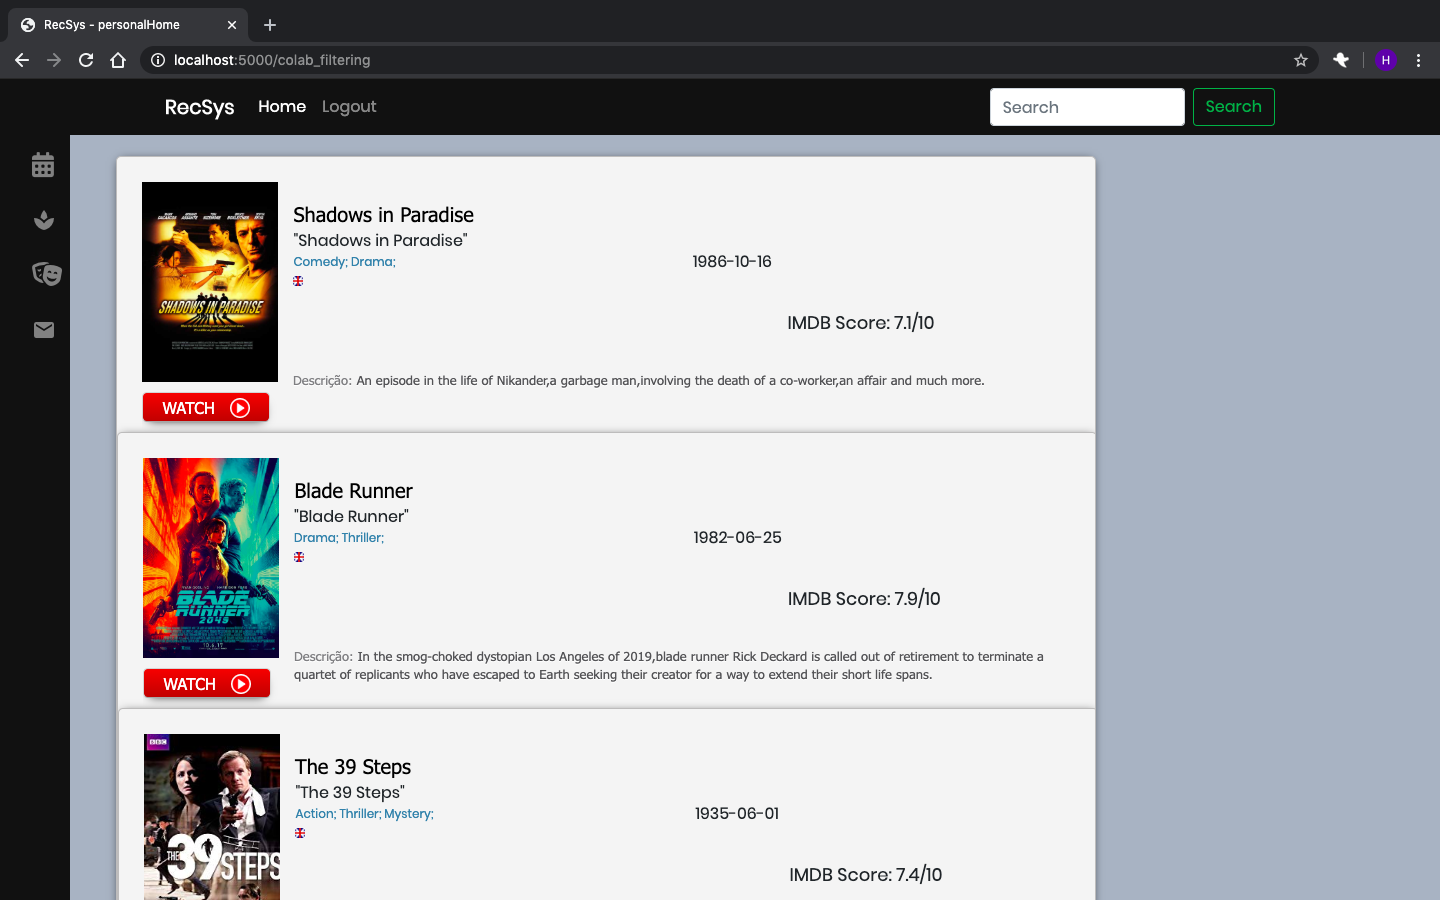
\includegraphics[scale=0.2]{colabFiltering.png}
\caption {Similar User's Views Page RecSys}
\label {fig15}
\end{figure}

Se escolhermos o sistema de recomendação \textit{"Your Personal List"} obtemos uma lista de filmes baseado nos géneros dos filmes vistos pelo utilizador. Esta lista resulta da aplicação do método filmWatchBased().\newline

\begin{figure}[H]
\centering
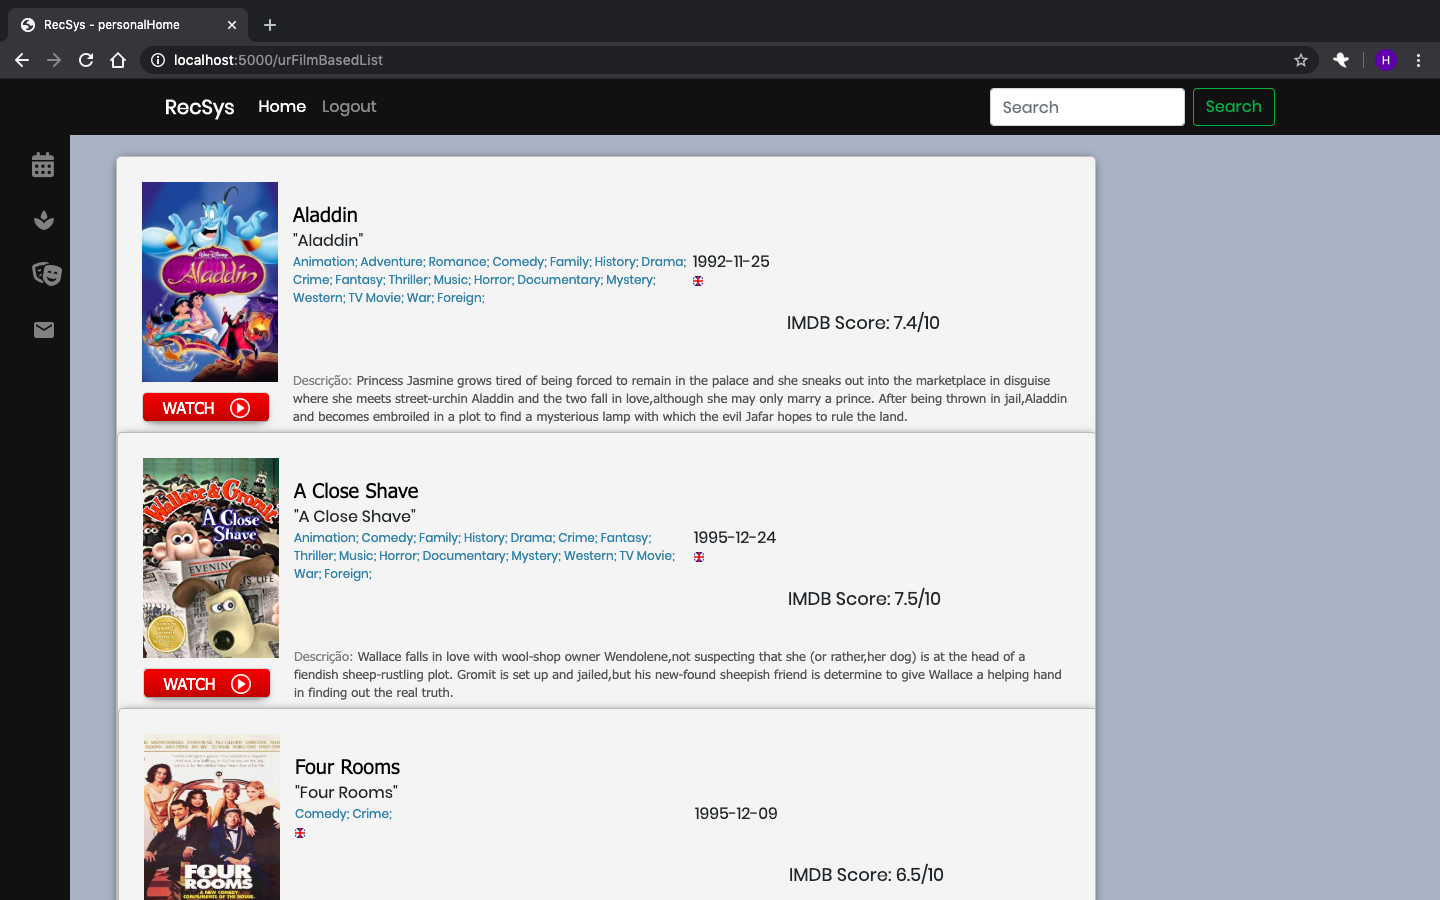
\includegraphics[scale=0.2]{watchedBased.png}
\caption {Your Personal List Page RecSys}
\label {fig16}
\end{figure}

Por fim, se escolhermos o sistema de recomendação \textit{"User's Best Rates"} obtemos uma lista dos filmes mais bem cotados por todos os utilizadores do sistema.\newline

\begin{figure}[H]
\centering
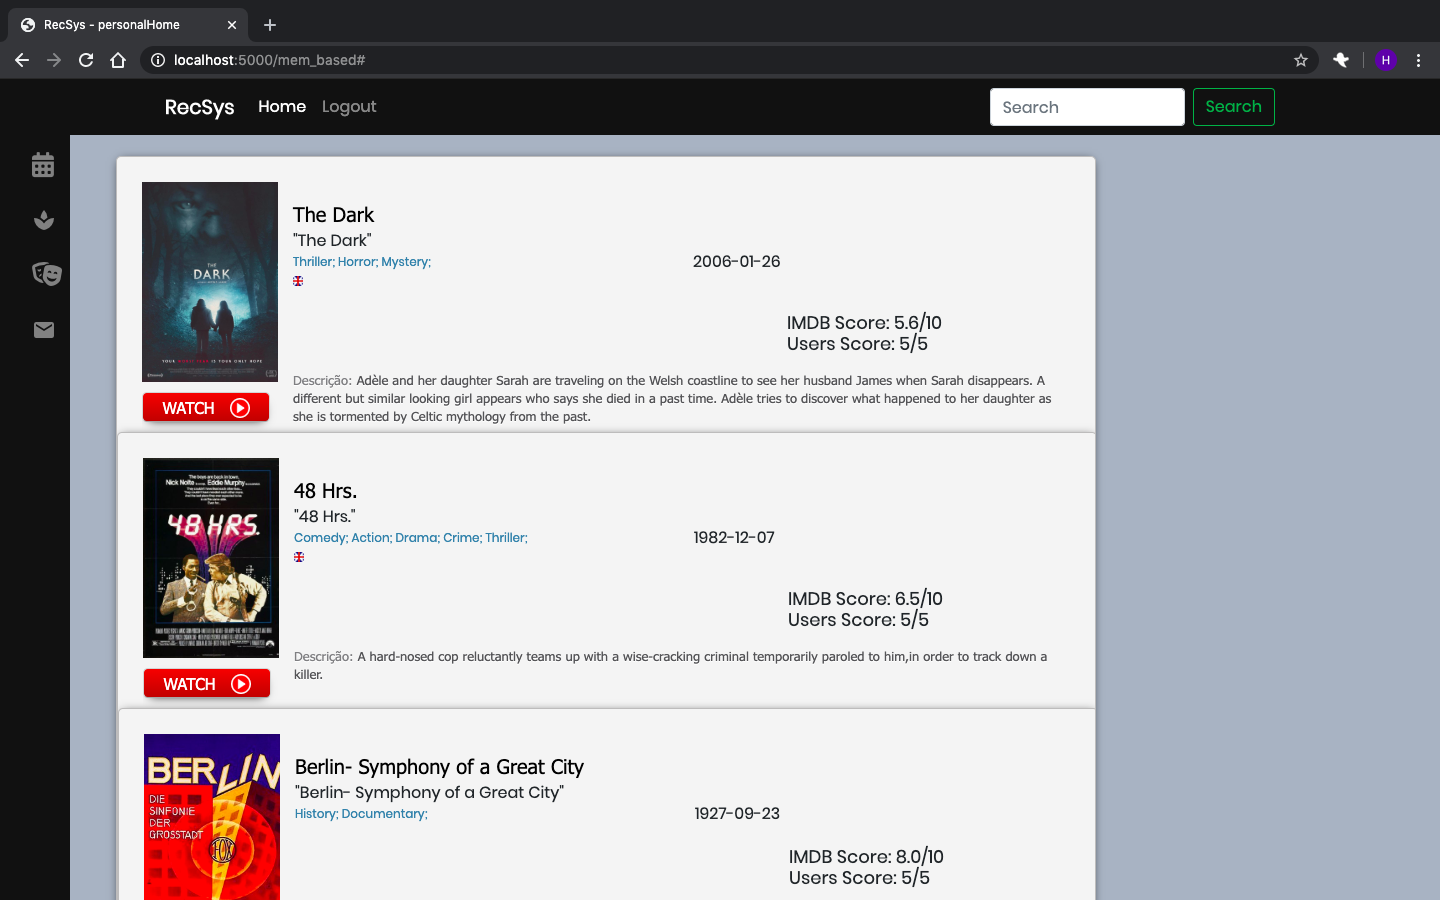
\includegraphics[scale=0.2]{user'sBestRates.png}
\caption {User's Best Rates Page RecSys}
\label {fig17}
\end{figure}

\newpage
